\begin{figure}[htbp]
\section*{ FGD1}
\centering
\begin{subfigure}[b]{0.95\textwidth}
\centering
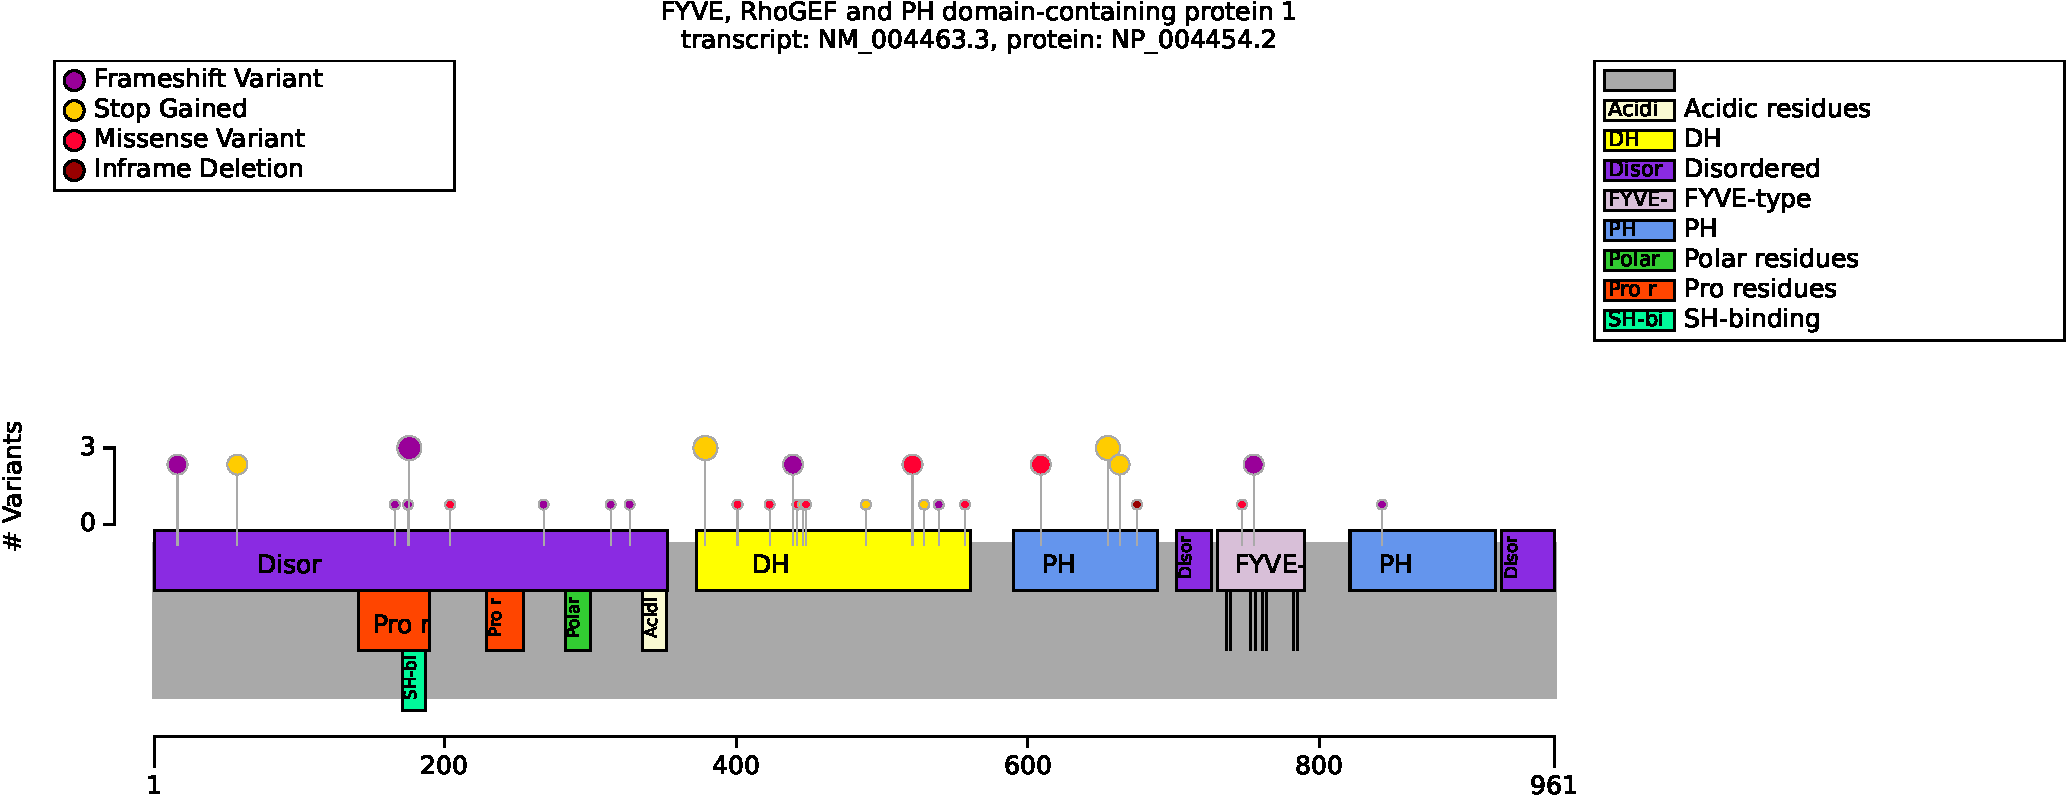
\includegraphics[width=\textwidth]{ img/FGD1_protein_diagram.pdf} 
\captionsetup{justification=raggedright,singlelinecheck=false}
\caption{Distribution of variants in FGD1}
\end{subfigure}

\vspace{2em}

\begin{subfigure}[b]{0.95\textwidth}
\centering
\resizebox{\textwidth}{!}{
\begin{tabular}{llllrr}
\toprule
Genotype (A) & Genotype (B) & total tests performed & significant results\\
\midrule
Missense & Other & 41 & 0\\
DH domain & Other & 43 & 0\\
\bottomrule
\end{tabular}
}
\captionsetup{justification=raggedright,singlelinecheck=false}
\caption{Fisher Exact Test performed to compare HPO annotation frequency with respect to genotypes. }
\end{subfigure}

\vspace{2em}

\caption{ The cohort comprised 16 individuals (0 females, 16 males). A total of 36 HPO terms were used to annotate the cohort. Disease diagnosis: Aarskog-Scott syndrome (OMIM:305400). No statistically significant results identified. A total of 16 unique variant alleles were found in \textit{FGD1} (transcript: \texttt{NM\_004463.3}, protein id: \texttt{NP\_004454.2}).}
\end{figure}
